\chapter{Generatorsystem für die Spreadshirt-API}
\label{chap:generator-system_for_spreadshirt-api}

\chapterQuote{An abstraction is one thing that represents several real things equally well.}{\citeauthor{Dijkstra}}{\citeyear{Dijkstra}}{\cite[][zitiert von David Lorge Parnas]{Dijkstra}}

Nachdem in den vorangegangen Kapiteln allgemeine Grundlagen über Webservices (\cref{chap:web_services}) und Codegenerierung (\cref{chap:codegeneration}) behandelt wurden, werden in diesem Kapitel die konkreten Datenmodelle, der Generator und der Aufbau der generierten Bibliothek für die Spreadshirt-\textsc{Api} beschrieben.

\section{Konkrete Datenmodelle}
\label{sec:concrete_models}

Neben den Datenmodellen, welche die Informationen beinhalten aus denen der Generator ausführbaren Quellcode erzeugt, wird im folgenden Abschnitt das im Sprachenmodell verwendete Kompositum-Muster erläutert.

\subsection{REST-Modell}
\label{sec:rest_model}

Zuerst muss die abstrakte Beschreibung der Spreadshirt-API von der XML-Form, bestehend aus einem \emph{WADL} (\cref{sec:wadl}) und einem oder mehreren Schemabeschreibungen (siehe \cref{sec:document_description_formats}), in ein für den Generator verarbeitbares Format überführt werden.

Die durch die WADL-Datei beschriebene Baumstruktur muss in ein Datenmodell bestehend aus Klassen und Objekten transformiert werden.
Um effektiv mit der XML Darstellung arbeiten zu können wird diese zuerst mit einem Parser (siehe \cref{sec:xml_parser}) in ein \emph{Document Object Model} (kurz DOM) überführt welches im Arbeitsspeicher gehalten wird und damit einen schnellen Zugriff für nachfolgende Operationen darauf erlaubt. In einem nächsten Schritt wird das DOM, welches noch viele XML spezifische Informationen enthält, auf die wesentlichen API beschreibenden Merkmale reduziert. Im Gegensatz zu der in \cref{fig:wadlstructure} veranschaulichten Webanwendungsbeschreibung werden Referenzen durch deren Definition im Modell ersetzt. Die Klassenamen des Datenmodells orientieren sich an den WADL Elementnamen.

\begin{figure}[tb]
    \centering
    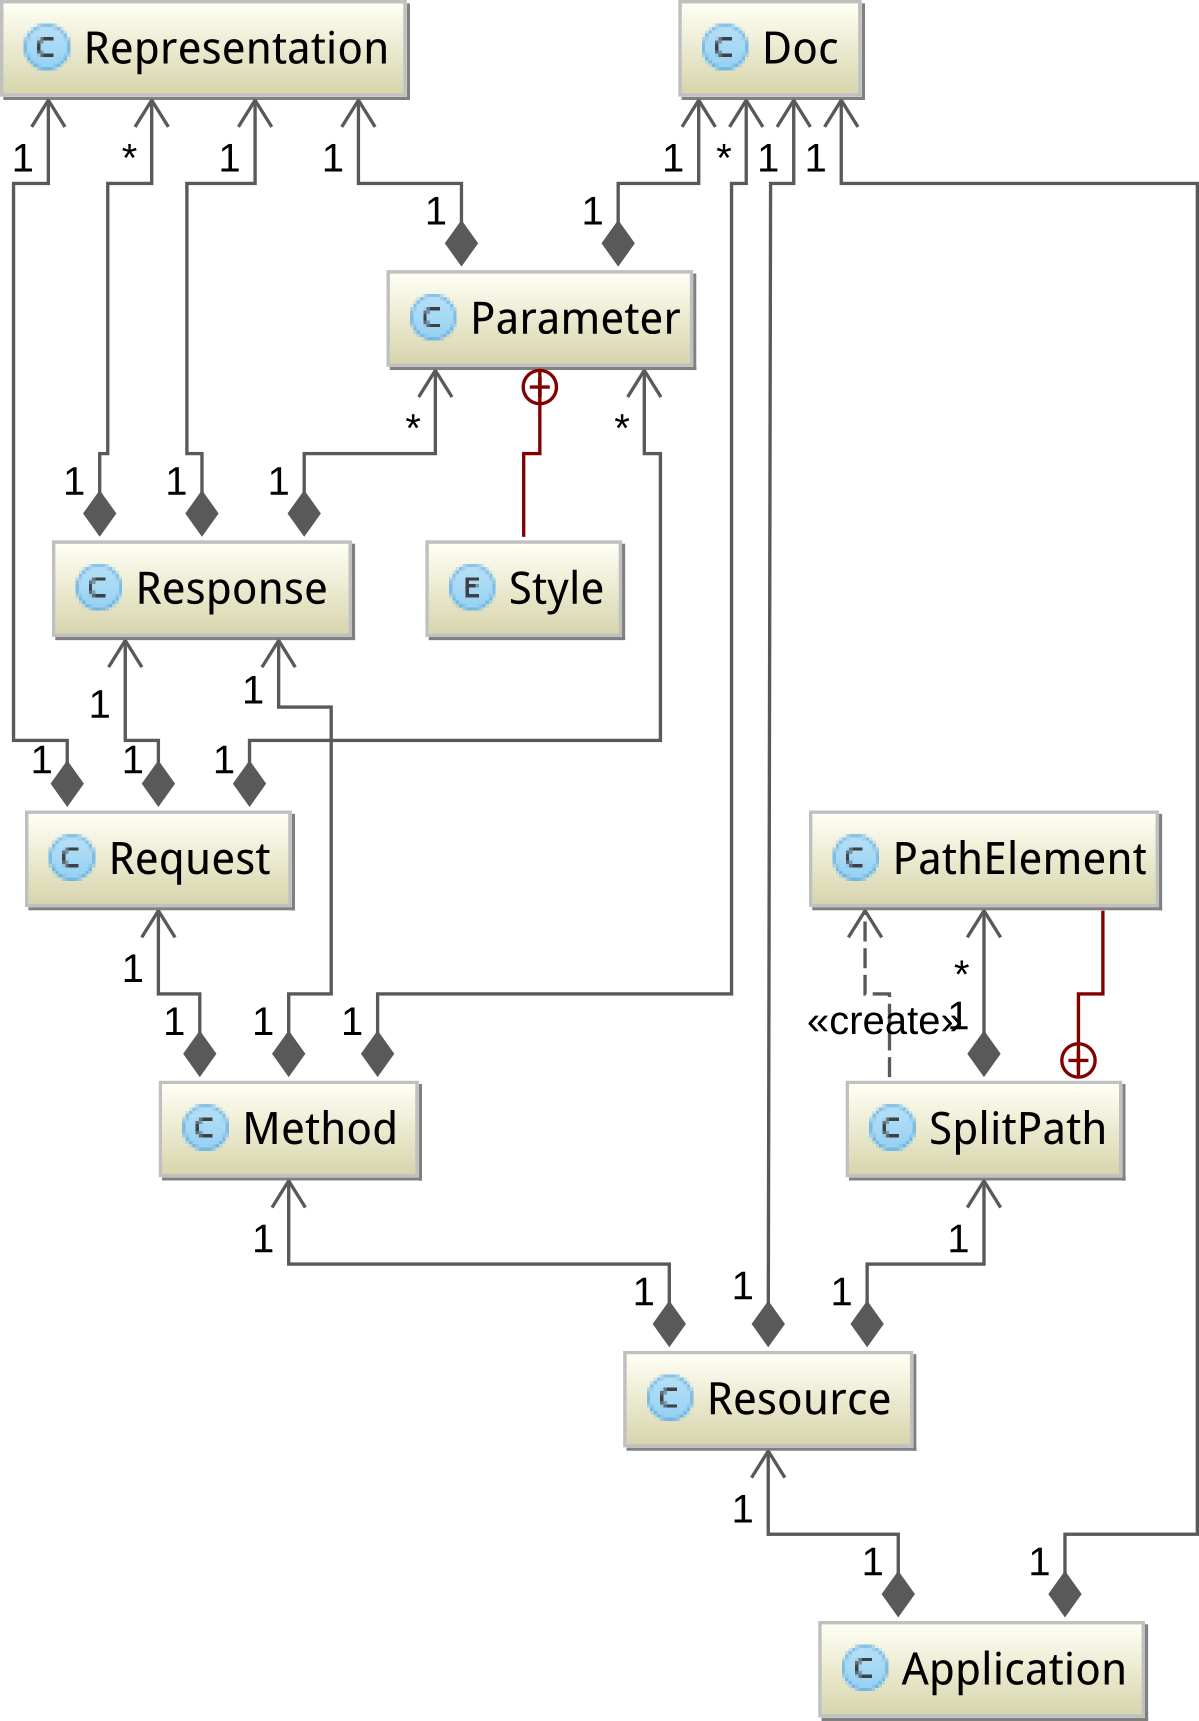
\includegraphics[width=0.5\textwidth]{resources/restmodel}
    \caption{UML Klassendiagramm des REST-Modells}
    \label{fig:restmodel}
\end{figure}

Wurzelelement des Modells (siehe \cref{fig:restmodel}) ist die Klasse \textbf{Application}, sie enthält \emph{Ressource}-Objekte und den Basisbezeichner der API bspw. \texttt{\small http://api.spreadshirt.net/api/v1/}. 

Eine \textbf{Ressource}-Klasse enthält eine Menge von \emph{Method}-Objekten, sowie einen Ressourcenbezeichner, dieser ist relativ zum Basisbezeichner des Wurzelelements. Die Ressourcenbezeichner können \emph{Template-Parameter} enthalten, diese werden bei einer Anfrage durch einen konkreten Wert ersetzt. Beispielweise enthält der Bezeichner für die Ressource eines bestimmten Users den Template-Parameter \{userid\}, vollständiger Ressourcenbezeichner \texttt{users/\{userid\}}. Ressourcenbezeichner werden durch die Klasse \textbf{SplitPath} repräsentiert. 

Jede \textbf{Method}-Klasse enthält ein \emph{Request} und ein \emph{Response} Objekt. Sie enthalten die nötigen Informationen für den Aufruf der Methode, bzw. über den Aufbau der Antwortnachricht.

Eine \textbf{Request}-Klasse enthält eine Liste von Query-Parametern sowie ein \emph{Representation} und \emph{Response} Objekt.

\textbf{Parameter} enthält Angaben zum \emph{Style}, Typ, Vorgabewert und ob dessen Angabe \enquote{required}, also notwendig ist. Die Angabe des Typs ist eine Referenz auf einen Typ aus einer XML-Schemabeschreibung. Der \emph{Style} gibt an wie der Parameter übermittelt wird, als Teil der Query \texttt{\ldots{}?mediaType=xml}, \emph{Key-Value Pair} des HTTP-Header oder als \emph{Template-Parameter} des Ressourcenbezeichners. 

Die Klasse \textbf{Response} enthält eine Liste mit \emph{Representation}-Objekten und Parameter-Objekten. Die Objekte vom Typ Representation enthalten die Beschreibung der Daten die bei einer erfolgreichen Anfrage an die Ressource zurückgesendet werden, sowie die der Fehlermeldung welche der Client anderenfalls erhält. Zwischen einer Fehlermeldung und einer erfolgreichen Anfrage kann anhand des Werts des HTTP-Statuscodes unterschieden werden. Erfolgreiche Anfragen liefern in der Antwort smeist einen Statuscode 200 \textbf{OK} oder 201 \textbf{Created} zurück, abhängig von der Anfragemethode. Die Response Parameter geben Einträge im HTTP-Header an, welche für den Client nützliche Informationen enthalten. Legt der Client z.B. via POST auf der Ressource \texttt{sessions} eine neue API-Session an, so enthält das Feld \texttt{Location} des HTTP-Headers der Serverantwort eine URL auf die Ressource der angelegten Session.

Die \textbf{Representation}-Klasse dient zur Beschreibung der Daten welche entweder zur API gesendet oder von dieser empfangen werden, sie besteht aus einer Angabe des \emph{media-type}, des HTTP-Statuscodes und eine Referenz auf die Definition des Datentyps. Das \emph{Representation}-Objekt des Request einer PUT- oder POST-Methode charakterisiert zum Beispiel den Aufbau der Daten welche der Ressource übermittelt werden, üblicherweise im HTTP-Body. Die Charakterisierung erfolgt dabei in Form einer Referenz auf einen Typ aus einer Schemabeschreibung sowie der Angabe des \emph{media-type}. Beispielsweise enthält das \emph{Representation}-Objekt der PUT-Methode auf Ressource \texttt{users/\{userId\}/designs/\{designId\}} den media-type \texttt{application/xml} und eine Referenz auf den Typ \texttt{sns:design}. 

Referenzen auf Typdeklaration aus einer Schemabeschreibung werden nachfolgend im Modell durch die konkrete Deklaration des Typs aus der XML-Schemabeschreibung ersetzt, siehe \cref{sec:application_model}. 

Ein Objekt der \textbf{Doc}-Klasse enthält einen Titel und eine Kurzbeschreibung des zugehörigen Elements.
Der Generator erzeugt daraus Quellcodekommentare für die Dokumentation der Bibliothek.

\subsection{Schema-Modell}
\label{sec:schema_model}

\begin{figure}[t]
    \centering
    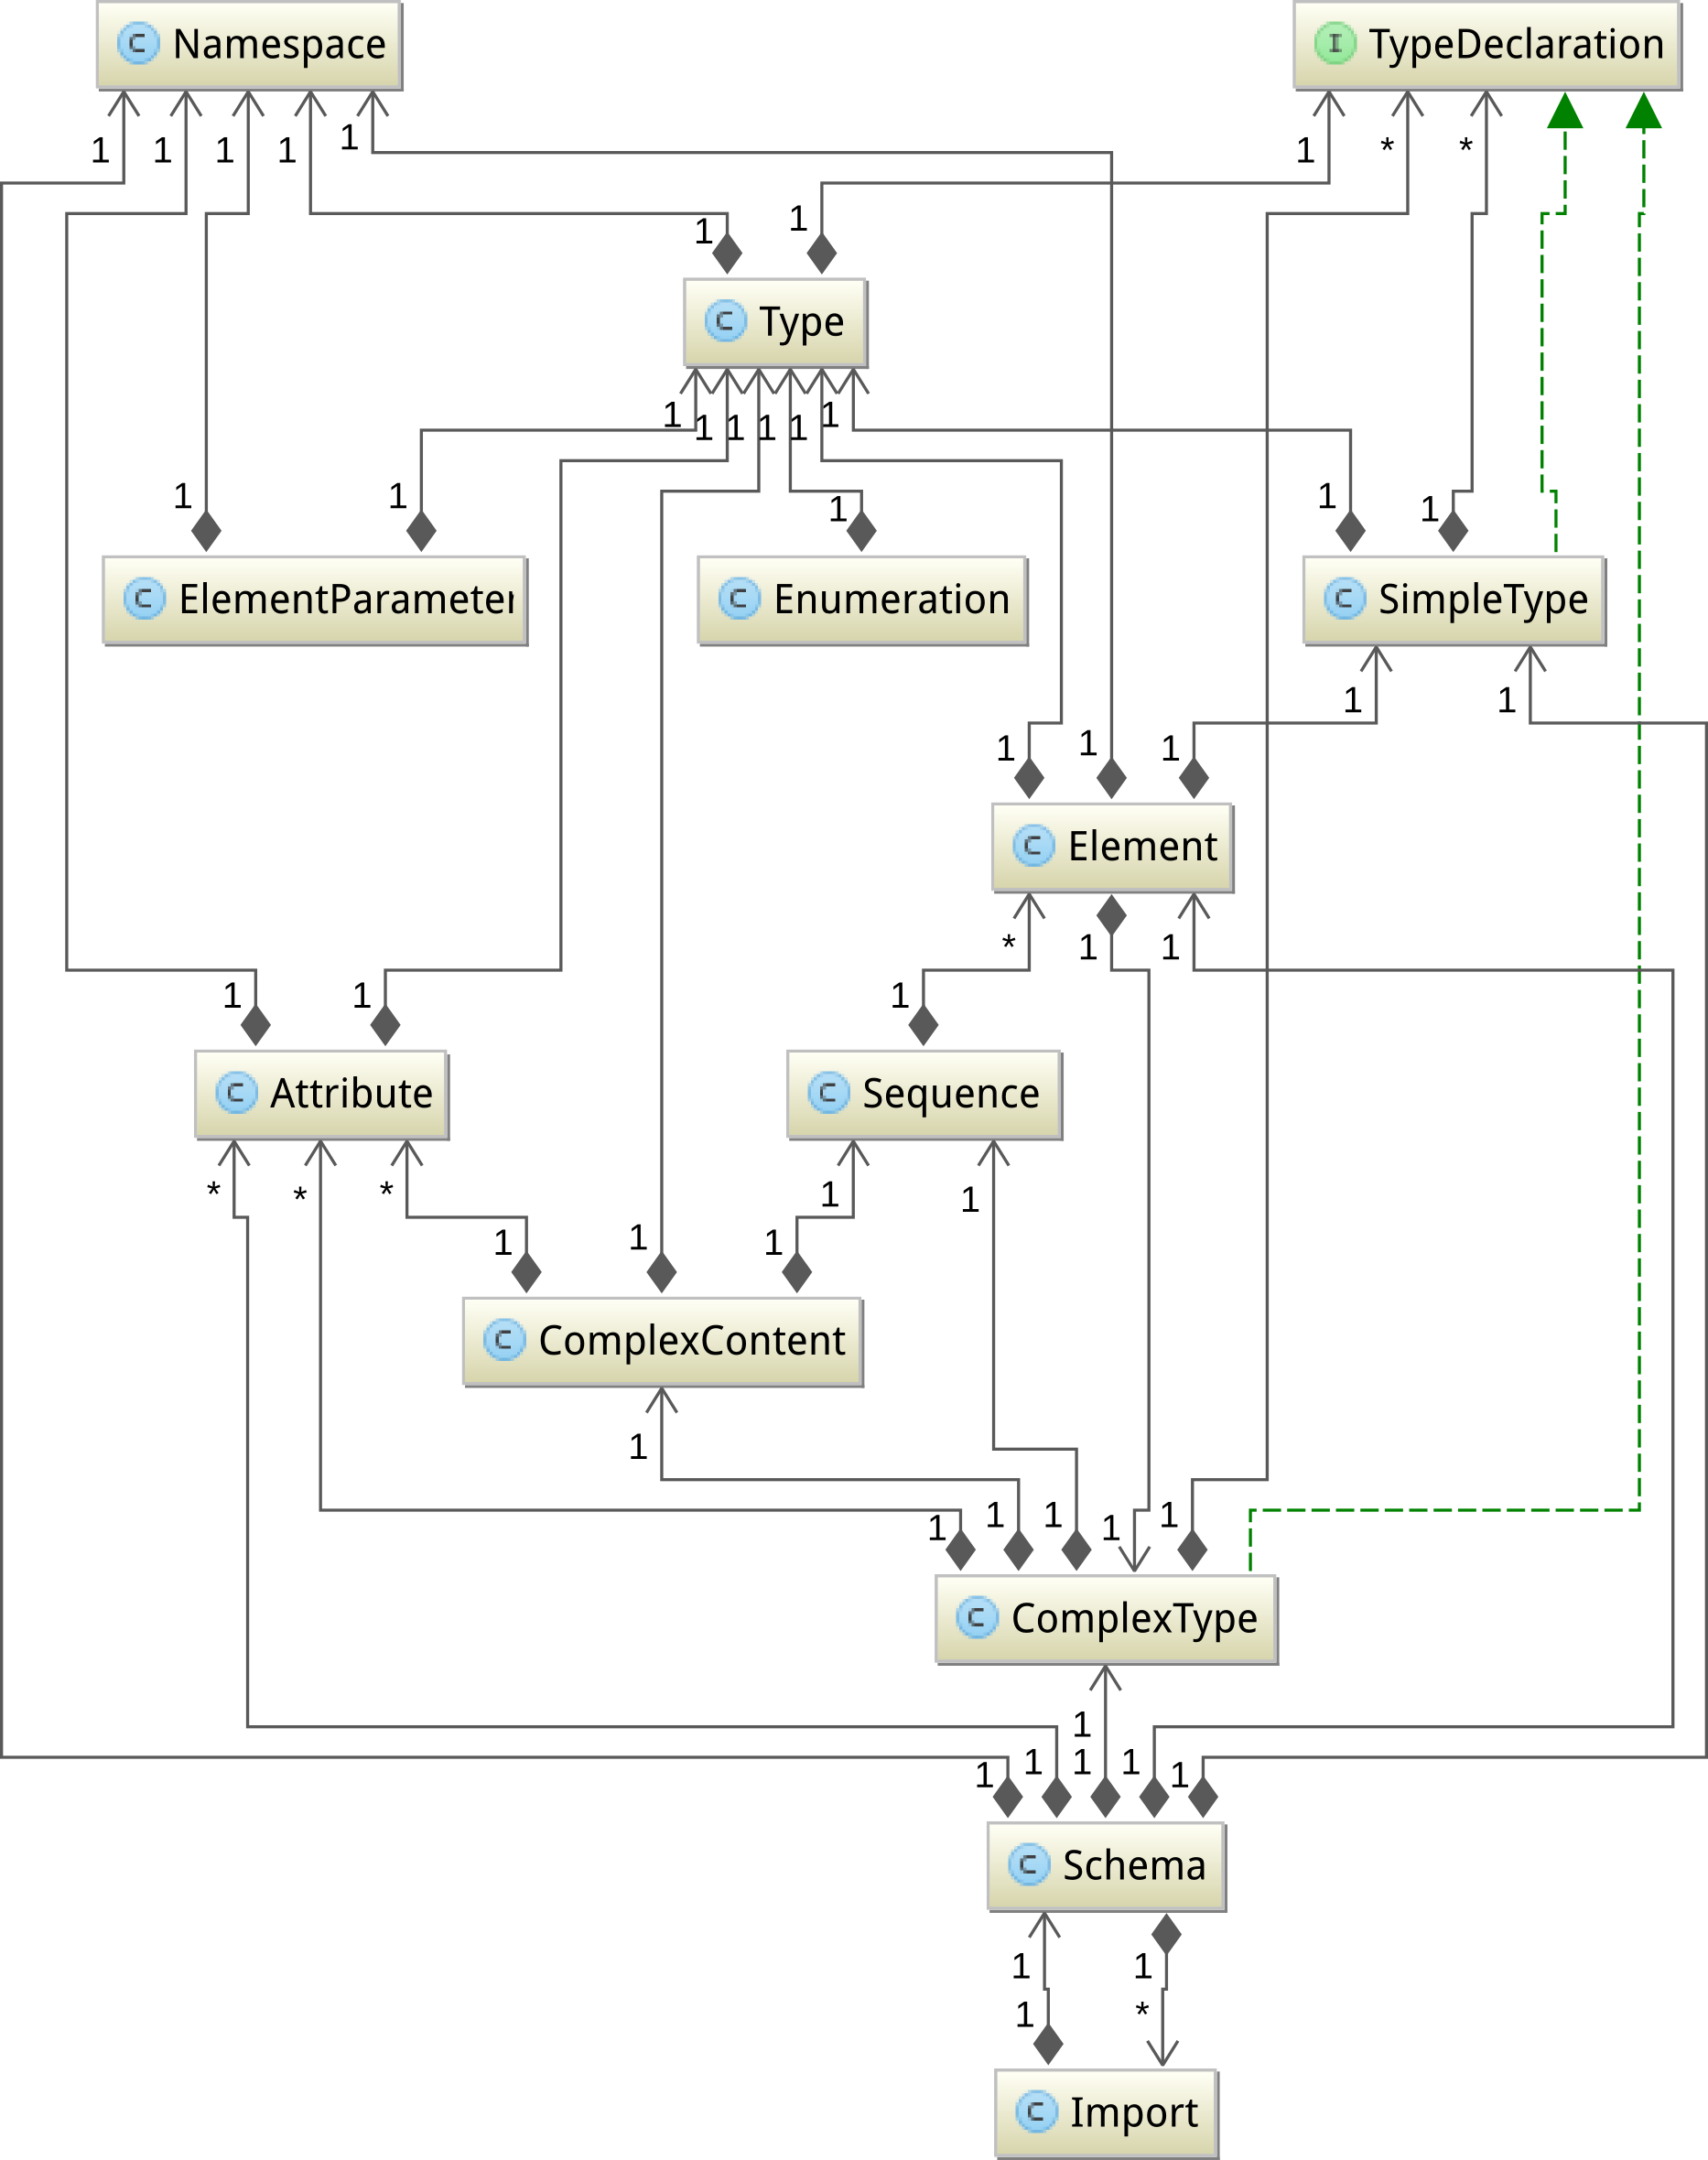
\includegraphics[width=0.6\textwidth]{resources/typemodel}
    \caption{\textsc{Uml} Klassendiagramm des Schemadatenmodells}
    \label{fig:schema_model}
\end{figure}

Wurzel des Schemadatenmodells ist die Klasse \textbf{Schema}. Ein Schema kann Objekte vom Typ \emph{Complex-} und \emph{SimpleType} sowie \emph{Attribute} und \emph{Element} enthalten.

\gls{XSD}-Dateien erlauben das Importieren anderer Schemadefinitionen, die Klasse \textbf{Import} ermöglicht dies im Schemamodell. Sie besitzt ein Objekt des zu importierenden Schemas sowie eine \gls{URI} auf die zugehörige \gls{XSD}-Datei.

Primitive Schematypen werden durch die Klasse \emph{SimpleType} abgebildet. Objekte dieser Klasse enthalten eine Kennzeichnung der Art des SimpleType (Enumerator, Liste, einfacher Wert) und bei Enumeratoren zusätzlich die einzelnen Enumeratorwerte sowie die Angabe des Basisdatentyps.

Die \textbf{ComplexType}-Klasse repräsentiert die gleichnamigen strukturierten Typen aus der Schemabeschreibung. 
Ein ComplexType kann Attribute, Elemente, Elementsequenzen und strukturierten Inhalt (\emph{ComplexContent}) enthalten.

\textbf{ComplexContent} kann die gleichen Objekte wie \emph{ComplexType} enthalten, sowie einen Basistyp der erweitert oder eingeschränkt wird (\enquote{derivation by extension/restriction}).

Attribute werden durch die gleichnamige Klasse \textbf{Attribute} gekapselt, sie besitzen einen Attributnamen sowie eine Definition ihres Typs.

Elementsequenzen werden durch die \textbf{Sequence}-Klasse repräsentiert. Sie enthält einen Reihenfolgeindikator und die Elemente der Sequenz.

Objekte der Klasse \textbf{Element} besitzen einen Bezeichner sowie einen Complex- oder SimpleType und optional eine Angabe der Auftrittshäufigkeit. Die Klasse \emph{ElementParameter} dient nur zur Kapselung der Daten, welche an den Konstruktor der Elementklasse gegeben werden.

Durch die Klasse \textbf{Namespace} werden der Namensraumbezeichner und der konkrete Namensraum eines Typs aus dem Schema gekapselt. 

\begin{figure}[ht]
    \centering
    \begin{minipage}[b]{0.6\linewidth}
        \begin{lstlisting}[
            language=XML,
            label=lst:xsdExamplePoint,                
            numbers=none,
            xleftmargin=0mm,
            framexleftmargin=2mm,
        ]
<xs:element 
    xmlns:tns="http://api.spreadshirt.net" 
    type="tns:point" name="point"/>

<xs:complexType name="point">
    <xs:sequence>
        <xs:element 
            type="xs:double" name="x"/>
        <xs:element 
            type="xs:double" name="y"/>
    </xs:sequence>
    <xs:attribute 
        xmlns:tns="http://api.spreadshirt.net" 
        type="tns:unit" name="unit"/>
</xs:complexType>
        \end{lstlisting}
    \end{minipage}
    \quad    
    \begin{minipage}[b]{0.35\linewidth}
        \begin{tikzpicture}[every tree node/.style={font=\footnotesize}]
            \Tree
            [
                .Element
                [
                    .ComplexType
                    [ . Attribute ]
                    [ .Sequence 
                        Element
                        [ .Element ]
                    ]
                ]
            ]
        \end{tikzpicture}
        %\label{fig:minipage2}
    \end{minipage}
    \caption{Datentyp Point mit Gegenüberstellung im Schemamodell}
\end{figure}

\subsection{Applikationsmodell}
\label{sec:application_model}

Das Applikationsmodell ist die Gesamtheit des \gls{REST}- und Schemamodells. Referenzen auf Typenbeschreibungen im \gls{REST}-Modell werden durch deren Definition im Schemamodell ersetzt. Dieses gemeinsame Modell dient dem Generator als Eingabequelle.

\subsection{Sprachenmodell}
\label{sec:language_model}

% Bild aktualisieren
\begin{sidewaysfigure}[tb]
    \centering
    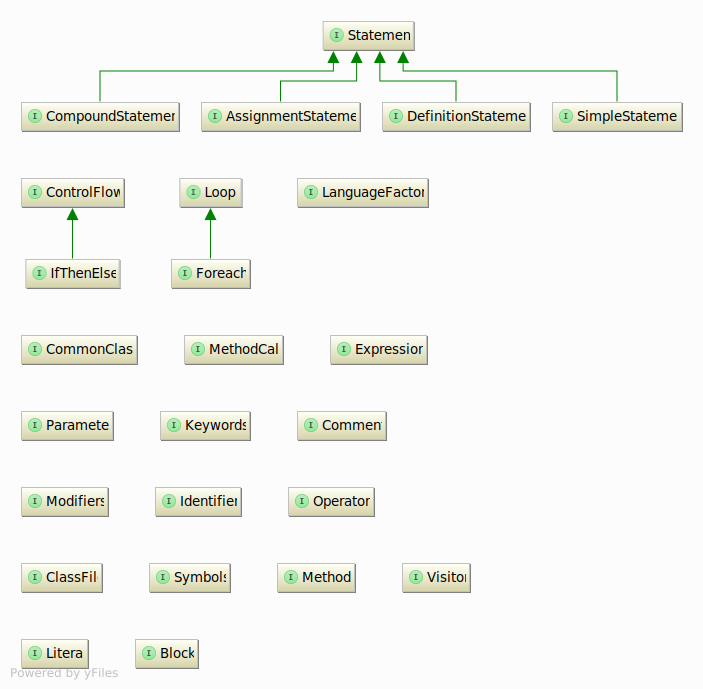
\includegraphics[width=\textwidth]{resources/languagemodel_common}
    \caption{UML Klassendiagramm des Zielsprachenmodells}
    \label{fig:language_model}
\end{sidewaysfigure}

Die Aufgabe des Generators ist die Transformierung des Applikationsmodells in das Modell der Zielsprache. 

Um die gewünschte Austauschbarkeit der Zielsprache zu gewährleisten wurde ein abstraktes Sprachenmodell entworfen welches die Konstrukte einer dateibasierten Objektorientierten Programmiersprache (siehe \cref{sec:oo_languages}) abbildet. 
%Anforderungen erstellen und referenzieren.
Die gewünschte Zielsprache muss dabei die Klassen und Methoden des Modells implementieren sowie eine \emph{Language Factory} (siehe \cref{sec:language_factory}) bereitstellen um vom Generator genutzt werden zu können.

Syntax ist kein Bestandteil des Modells sondern wird von einem \emph{LanguageVisitor} (siehe \cref{sec:language_visitor}) implementiert, das Sprachenmodell enthält nur die nötigen \emph{accept}-Methoden für den Visitor.

Basis des Modells ist die Klasse \textbf{ClassFile}, sie abstrahiert eine Klassendatei mit den Eigenschaften:
\begin{compactitem}
    \item Dateiname
    \item Namensraum
    \item Liste von Abhängigkeiten (\emph{Dependency}-Klasse)
    \item Klassendefinition
\end{compactitem}

Die Liste von Abhängigkeiten der zu generierenden Klassen muss vorher aus dem Eingabemodell ermittelt werden, dies geschieht durch Analyse der in den Elementdefinitionen des Schemamodells enthaltenen Typen. 

% Modifier sind Schlüsselwörter einer Sprache die deren Verhalten ändern.

\textbf{Keywords} und \textbf{Symbols} dienen zur Kapselung der Schlüsselwörter und Symbole einer Sprache. Keywords enthält Methoden zur Abfrage typischer Schlüsselworte wie \emph{class}, \emph{import}, \emph{new} oder \emph{this}. Sprachspezifische Symbole wie \emph{Verkettungs}- und \emph{Scope}-Operatoren oder Präfixe für Variablennamen können über Methoden der Klasse Symbols vom Generator abgefragt werden.

\subsection{Language Visitor}
\label{sec:language_visitor}

Kapitel gehört eher zu Generator

% Sprachschnittstelle!
\subsection{Language Factory}
\label{sec:language_factory}

Um eine Zielsprachenunabhänhigkeit zu erreichen, wird dem Generator bei der Erzeugung eine \enquote{Language Factory} übergeben. Der Generator erzeugt Sprachelemente nur über diese Factory. Ein Aufruf einer Factorymethode gibt ein Element der vom Typ der Sprache zurück, der Generator kennt aber nur den Interface-Typ. Für ihn ist die konkrete Implementierung somit transparent.


\section{Codegenerator}
\label{sec:codegenerator}

Nachdem in \cref{sec:concrete_models} die Datenmodelle des Generators betrachtet wurden, widmet sich dieser Abschnitt nur dem Aufbau des Codegenerators und den dort verwendeten Entwurfsmustern, \emph{Factory} (\cref{sec:language_factory}) und \emph{Visitor} (\cref{sec:language_visitor}). \Cref{fig:generation_process} zeigt ein Ablaufdiagramm des Generators.

\begin{sidewaysfigure}
    \centering
    \resizebox{ \textwidth}{!}{
        \begin{tikzpicture}[
        node distance=12mm and 8mm,
        every node/.style={font=\scriptsize}
    ]
    % Blocks
    \node(abstractDescription)[greyBlock]{Abstrakte\\Beschreibung\\der Spreadshirt-API};
    \node(dummy1)[dummy, right=of abstractDescription]{};
    \node(wadlAnalysis)[greyBlock, above right=of abstractDescription]{Analyse\\WADL-Datei};
    \node(restModel)[greyBlock, right=of wadlAnalysis]{REST-\\Modell};
    \node(xsdAnalysis)[greyBlock, below right=of abstractDescription]{Analyse\\XSD-Datei};
    \node(schemaModel)[greyBlock, right=of xsdAnalysis]{Schema-\\Modell};
    \node(modelCombine)[greyBlock, right=of dummy1]{Kombinierer};
    \node(applicationModel)[greyBlock, right=of modelCombine]{Applikations-\\Modell};
    \node(generator)[greyBlock, right=of applicationModel]{Generator};
    \node(languageModel)[greyBlock, right=of generator]{Zielsprachen-\\Modell};
    \node(languageFactory)[greyBlock, below=of generator]{Language Factory};
    \node(filePrinter)[greyBlock, right=of languageModel]{File Printer};
    \node(library)[greyBlock, double copy shadow, right=of filePrinter]{Bibliotheks-\\Dateien};

    %\node(languagemodel)[greyBlock, right= of generator]{Sprachenmodell\\\emph{Abstrakter Syntaxbaum}};
    % Lines  
    \path[arrow, ->] (abstractDescription) -- (wadlAnalysis);
    \path[arrow, ->] (abstractDescription) -- (xsdAnalysis);
    \path[arrow, ->] (wadlAnalysis) -- (restModel);
    \path[arrow, ->] (xsdAnalysis) -- (schemaModel);
    \path[arrow, ->] (restModel) -- (modelCombine);
    \path[arrow, ->] (schemaModel) -- (modelCombine);
    \path[arrow, ->] (modelCombine) -- (applicationModel);
    \path[arrow, ->] (applicationModel) -- (generator);
    \path[arrow, ->] (languageFactory) -- (generator);
    \path[arrow, ->] (generator) -- (languageModel);
    \path[arrow, ->] (languageModel) -- (filePrinter);
    \path[arrow, ->] (filePrinter) -- (library);

    %\path[arrow, ->] (infrastructurecode) -- (generator);
\end{tikzpicture}

    } 
    \caption{Ablaufdiagram des Generators}
    \label{fig:generation_process}
\end{sidewaysfigure}

\subsection{Language Factory}
\label{sec:language_factory}

Das \emph{Factory}-Pattern behandelt das Problem Familien von Objekten erzeugen zu wollen ohne die konkreten Klassen zu spezifizieren, sondern nur Interfaces festzulegen \cite[][S. 26]{patternsKompakt}.
Um eine Zielsprachenunabhängigkeit zu erreichen, wird dem Generator bei der Erzeugung eine Factory übergeben die das Interface \emph{Language Factory} des Sprachenmodells implementiert. 

Der Generator erzeugt Sprachelemente nur über diese Factory. Ein Aufruf einer Factorymethode gibt ein Sprachelement der Zielsprache zurück, der Generator kennt aber nur den Interface-Typ. Für ihn ist die konkrete Implementierung somit transparent. 
Die \emph{Language Factory} bildet damit die Schnittstelle zwischen dem Generator und der Implementierung des Zielsprachenmodells.

\subsubsection{Language Visitor}
\label{sec:language_visitor}

\citeauthor{patternsKompakt} definieren den Verwenduszweck des Patterns in \cite[][S. 60]{patternsKompakt} so: 
\thesisquote{Dieses Pattern ermöglicht es, neue Operationen auf den Elementen einer
Struktur zu definieren, ohne die Elemente selbst anzupassen.}

Die Aufgabe des \emph{Language Visitor} im Generator ist die Transformation des Sprachenmodells in eine Zeichenketten-Darstellung. Wie in \cref{sec:language_model} schon erwähnt, enthält die Klasse die das \emph{LanguageVisitor}-Interface implementiert, Regeln für eine syntaktisch korrekte Ausgabe des Sprachenmodells. Zusätzlich können in den LanguageVisitor \enquote{code conventions} implementiert werden, bspw. Einrückungstiefen, Zeilenlängen etc.

\subsection{Ausgabemodul}
\label{sec:printer_module}

Das Ausgabemodul beinhaltet Methoden zur Speicherung der Zeichenkettendarstellung aus dem \emph{Language Visitor}. Üblicherweise ist dies die Speicherung in Dateiform, es ist aber ebenso die Ausgabe auf \texttt{stdout} oder die Speicherung in einer Datenbank möglich.

\section{Client-Bibliothek}
\label{sec:client_library}

Die generierte Client-Bibliothek lässt sich in 2 verschiedene Arten von Klassen gliedern:
\begin{compactenum}
    \item die Elemente und Typen aus der \gls{XML}-Schemabeschreibung repräsentieren (\emph{Datenklassen});
    \item die \gls{API}-Ressourcen und deren Methoden abbilden (\emph{Ressourcenklassen}).
\end{compactenum}

Zusätzlich wurden für Aufgaben die keiner explizite Generierung bedürfen, wie \gls{HTTP}-Methodenaufrufe, manuell Klassen mit statischen Methoden erstellt. Dem Generator werden die Klassen als Abhängigkeiten im Eingabemodell bekannt gegeben und an enstprechender Stelle durch ihn als \emph{Import}-Anweisungen in der Bibliothek eingefügt. Keine explizite Generierung wird benötigt wenn der zu erzeugende Code keine oder sehr wenig variable Bestandteile enthält.

\subsection{Datenklassen}
\label{sec:dataclasses}

Die Datenklassen sind die zielsprachenabhängige Repräsentation der Elemente und Typen aus der \gls{XML}-Schemabeschreibung. 

Der Name der Klasse entspricht dabei der Bezeichnung des Typs oder des Elements. Die Variablen einer solchen Klasse sind die Attribute und Elemente aus der Schemabeschreibung des Typs. \textsc{Php} bietet keine Enumeratoren, deshalb werden die einzelnen Enum-Werte als statische Variablen vom Typ \texttt{string} generiert. Für alle Variablen werden außerdem Getter- und Setter-Methoden durch den Codegenerator erzeugt.

Konstruktoren zur Erzeugung von Objekten aus den Datenklassen werden ebenfalls vom Generator erstellt. Dabei werden die \emph{Häufigkeitsindikatoren} aus der Schemabeschreibung berücksichtigt. Bei einem \texttt{minOccurs}-Wert größer eins wird das Element zu den Konstruktor-Parametern hinzugefügt. Somit ist sichergestellt, dass notwendigen Angaben auch Werte zugeordnet werden.

Methoden zur De-/Serialisierung (\cref{sec:serialiser}) in eine der beiden von der Spreadshirt-\gls{API} unterstützten Dokumentbeschreibungsformate (\gls{JSON}, \gls{XML}) sind ebenfalls Bestandteil einer Datenklasse.

\Cref{lst:generatedDataClass} zeigt einen gekürzten Ausschnitt der generierten Datenklasse zum Element \emph{Point} aus der Schemabeschreibung der Spreadshirt-\gls{API}.

\subsection{Ressourcenklassen}
\label{sec:ressourceclasses}

Ressourcenklassen sind die zielsprachenabhängige Abbildung der Ressourcenbeschreibungen aus WADL-Datei der Spreadshirt-\gls{API}.

Eine Ressourcenklasse beinhaltet:
\begin{compactitem}
    \item[\ding{202}] ein Feld, welches die Basis-\gls{URL} der API beinhaltet;
    \item[\ding{203}] ein Feld in welches die komplette \gls{URL}, inklusive der ersetzten Template-Parameter (\cref{sec:rest_model}), der Ressource erhält;
    \item[\ding{204}] eine Menge von Feldern, die jeweils einem Template-Parameter zugeordnet sind;
    \item[\ding{205}] einen Konstruktor, dessen Argumente den Template-Parametern entsprechen und der aus diesen und der Basis-\gls{URL} die Ressourcen-\gls{URL} erstellt;
    \item[\ding{206}] Abbildungen der Methoden aus der Ressourcenbeschreibung. Methodenparameter, die zur Authentifizierung an der \gls{API} notwendig sind, werden durch einen Parameter der Klasse \emph{ApiUser} (\cref{sec:api_auth}) substituiert \ding{207}.
\end{compactitem}

\Cref{lst:generatedRessourceClass} beinhaltet die generierte Klasse zur Ressource \texttt{users/{userId}/products} der Spreadshirt-\gls{API}.

\begin{lstlisting}[
    language=PHP,
    caption=Point-Klasse als (gekürztes) Beispiel für eine generierte Datenklasse,
    label=lst:generatedDataClass
]
<?php
   require_once('Unit.php');

   class Point
   {
      private $unit; // unit 
      private $y; // double 
      private $x; // double 

      function __construct(
            /* double */ $y,
            /* double */ $x
         )
      {
         $this->y = $y;
         $this->x = $x;
      }

      public function setUnit(
            /* unit */ $unit
         )
      {
         $this->unit = $unit;
      }

      public function toJSON()
      {
         $json = json_decode(/* Point */ $this);
         return $json;
      }

      public function toXML()
      {
         $xml =  new SimpleXMLElement(/* Point */ '<login xmlns="http://api.spreadshirt.net"/>');
         $xml->addChild(/* string */ 'unit',/* unit */ $this->unit);
         $xml->addChild(/* string */ 'y',/* double */ $this->y);
         $xml->addChild(/* string */ 'x',/* double */ $this->x);
         return $xml->asXML();
      }

      public static function fromXML(
            /* SimpleXMLElement */ $xml
         )
      {
         $unit = Unit::fromXML(/* SimpleXMLElement */ $xml->unit);
         $y = $xml->y;
         $x = $xml->x;
         $Point =  new Point(/* double */ $y,/* double */ $x);
         $Point->setUnit(/* unit */ $unit);
         return $Point;
      }

      ...

      public function getX()
      {
         return $x = $this->x;
      }
   }
?>
\end{lstlisting}

\newpage

\begin{minipage}{\textwidth}
\begin{lstlisting}[
    language=PHP,
    caption=Klasse zur Ressource \texttt{users/{userId}/products} als Beispiel für eine Ressourcenklasse,
    label=lst:generatedRessourceClass
]
<?php
   require_once('Static/methods.php'); //@\label{lst:importMethods}@//
   require_once('Static/apiUser.php'); //@\label{lst:importApiUser}@//

   /* Create or list products for user. */
   class UsersUserIdProducts
   {
      private $baseUrl = 'http://192.168.13.10:8080/api/v1/'; // string //@\ding{202}@//
      public $userId; // string //@\ding{204}@//
      private $resourceUrl = ''; // string //@\ding{203}@//

      /*  */
      public function POST( //@\ding{206}@// //@\label{lst:methodParameters}@//
            /* array */ $parameters, 
            /* ApiUser */ $apiUser,
            /* ProductDTO */ $productDTO
         )
      {
         $auth = $apiUser->getAuthentificationHeader(/* string */ 'POST',/* string */ $this->resourceUrl);
         return Methods::post(/* string */ $this->resourceUrl,/* string */ $auth,/* array */ $parameters,/* ProductDTO */ $productDTO); //@\label{lst:staticMethodPost}@//
      }

      /* Sample Url is:  http://... */
      public function GET( //@\ding{206}@//
            /* array */ $parameters,
            /* ApiUser */ $apiUser //@\ding{207}@//
         )
      {
         $auth = $apiUser->getAuthentificationHeader(/* string */ 'GET',/* string */ $this->resourceUrl);
         return Methods::get(/* string */ $this->resourceUrl,/* string */ $auth,/* array */ $parameters); //@\label{lst:staticMethodGet}@//
      }

      function __construct( //@\ding{205}@//
            /* string */ $userId
         )
      {
         $this->userId = $userId;
         $this->resourceUrl = $this->baseUrl . 'users' . '/' . $userId . 'products';
      }
   }
?>
\end{lstlisting}
\end{minipage}

\subsection{De-/Serialisierer}
\label{sec:serialiser}
% todo: transportunabhängig als Schlagwort entfernen?

Um \emph{Ressourcen-Repräsentationen} (\cref{sec:representation}) mit der Spreadshirt-\gls{API} transportunabhängig austauschen zu können, müssen die strukturierten Datenklassen \emph{serialisiert} werden. In umgekehrter Richtung müssen \emph{Repräsentation} aus der \gls{API} deserialisiert --- also wieder in eine Datenklasse transformiert --- werden.

Die Datenklassen-Methoden zur Serialiserung und Deserialiserung besitzen einheitliche Bezeichner, nach dem Schema \texttt{toXML}, \texttt{toJSON}, respektive \texttt{fromXML}, \texttt{fromJSON}. Die Deserialisierer-Methoden sind \emph{statisch} um das unnötige Instanziieren einer Datenklasse zu vermeiden, nur um ihre Klassendarstellung aus der serialisierten Form zu erhalten.

Beispiele für beide Arten finden sich in \Cref{lst:generatedDataClass}.

\subsection{Statische Klassen}
\label{sec:static_classes}

\emph{Statische Klassen} bedeutet in dem Codegenerierungskontext, dass diese \emph{manuell} erstellt wurden. Die statischen Klassen enthalten Code der von anderen Klassen gemeinsam genutzt wird und keine variablen Bestandteile enthält. 

Prinzipiell werden zwei Probleme durch statische Klassen vermindert:
\begin{compactenum}
  \item unnötige Vergrößerung des generierten Codes
  \item Vermeidung des Aufwands zur Implementierung der statischen Inhalte in dem Eingabemodell des Generators
\end{compactenum}

Die generierte Client-Bibliothek beinhaltet dabei zwei dieser Klassen:
\begin{compactenum}
  \item zur Kommunikation mit der \gls{API} über \gls{HTTP}-Methoden
  \item zur Kapselung von Authentifizierungsinformationen
\end{compactenum}

Den Import beider Klassen zeigt \Cref{lst:generatedRessourceClass} in Zeile~\ref{lst:importMethods} und~\ref{lst:importApiUser}.

\subsubsection{Nutzung der HTTP-Methoden}
\label{sec:staticMethodsClass}

Um die generierten Ressourcenklassen nicht unnötig zu vergrößern wurde der \emph{einheitliche} Vorgang zum Aufruf der \gls{HTTP}-Methoden in eine manuell erstellte Klasse ausgelagert.

\Cref{lst:generatedRessourceClass} zeigt in Zeile~\ref{lst:staticMethodPost} und~\ref{lst:staticMethodGet} den Aufruf zweier solcher Methoden aus einer Ressourcenklasse.

\subsubsection{API Authentifizierung}
\label{sec:api_auth}

In der Spreadshirt-\gls{API} sind geschützte und ungeschützte Ressourcen vorhanden. 

Das zur Authentifizierung eines \gls{API}-Nutzers verwendete Protokoll \emph{SprdAuth} basiert auf \enquote{\gls{HTTP}s Authorization Request Header} sowie dem \enquote{\textsc{Www}-Authentificate Response Header} \cite{apiSecurity}.

Die Spreadshirt-\gls{API} unterstüzt die Übergabe der nötigen Autorisierungsparameter als Teil der \gls{URI}-Query oder in Form des \emph{Authorization-Header}. Die erzeugte Client-Bibliothek beschränkt sich auf die Nutzung des \emph{Authorization-Headers}, dieser besitzt folgenden Aufbau:

\begin{lstlisting}[
    language=JavaScript,
    caption=Aufbau des Spreadshirt Authentification Header,
    label=lst:authHeader
]
Authorization:  SprdAuth apiKey="<apikey>", //@\ding{202}@// 
                data="<method> <url> <time>", 
                sig="SHA1(<method> <url> <time> <secret> //@\ding{203}@// )", 
                sessionId="<sessionId>" //@\ding{204}@//
\end{lstlisting}

Die Klasse \classname{ApiUser} kapselt die Daten, die zur Autorisierung an der \gls{API} nötig sind und stellt eine Methode bereit, die dem Nutzer das Erstellen des Authorization-Headers erspart. Der Konstruktor der ApiUser-Klasse erwartet dabei die Angabe der folgenden Parameter:

Alle Methoden, die eine Autorisation benötigen erhalten vom Codegenerator einen Parameter vom Typ \emph{ApiUser} wie \ding{206} in \Cref{lst:generatedRessourceClass} zeigt.

\begin{compactitem}
    \item \emph{UserID}, die Indentifikationsnummer des Spreadshirt-Nutzers
    \item \emph{ApiKey} und \emph{Secret} (\ding{202}, \ding{203}), diese Informationen erhält der Nutzer, wenn er sich als \gls{API}-User bei Spreadshirt registriert
    \item \emph{SessionID} (\ding{204}), die SessionID ist in der Response der POST-Methode auf Ressource \texttt{sessions} enthalten.
\end{compactitem}


%\section{API-Design}
\label{sec:api-design}

\subsection{Kriterien}
\label{sec:design_criterias}

\subsection{Sessions}
\label{sec:sessions}

\subsection{Parameterobjekte}
\label{sec:parameter_objects}

\subsection{Entwurfsmuster}
\label{sec:patterns}

\subsubsection{Expression Builder}
\label{sec:expression_builder}

\subsubsection{Fluent Interface}
\label{sec:fluent_interface}

